\documentclass[conference]{IEEEtran}
\IEEEoverridecommandlockouts

\usepackage{cite}
\usepackage{amsmath,amssymb,amsfonts}
\usepackage{algorithmic}
\usepackage{graphicx}
\usepackage{textcomp}
\usepackage{xcolor}
\usepackage{hyperref}
%% ODE handling
\usepackage{diffcoeff}
\usepackage{booktabs}
%% The SI units alignment
\usepackage{siunitx}
\def\BibTeX{{\rm B\kern-.05em{\sc i\kern-.025em b}\kern-.08em
    T\kern-.1667em\lower.7ex\hbox{E}\kern-.125emX}}
\begin{document}

\title{Integrating Weather Forecasts and Energy Management in Lettuce Growth: A Model Predictive Control Framework for Precision Agriculture
    \thanks{This research is funded by the Slovak Research and Development Agency under the project APVV-21-0019, by the Scientific Grant Agency of the Slovak Republic under the grant 1/0691/21, and by the European Commission under the grant no. 101079342 (Fostering Opportunities Towards Slovak Excellence in Advanced Control for Smart Industries).}
}

\author{\IEEEauthorblockN{Marek Wadinger}
    \IEEEauthorblockA{\textit{Faculty of Chemical and Food Technology} \\
        \textit{Slovak University of Technology in Bratislava}\\
        Bratislava, Slovakia \\
        marek.wadinger@stuba.sk}
    \and
    \IEEEauthorblockN{Erika Pavlovičová}
    \IEEEauthorblockA{\textit{Faculty of Chemical and Food Technology} \\
        \textit{Slovak University of Technology in Bratislava}\\
        Bratislava, Slovakia \\
        erika.pavlovicova@stuba.sk}
    \and
    \IEEEauthorblockN{Rastislav Fáber}
    \IEEEauthorblockA{\textit{Faculty of Chemical and Food Technology} \\
        \textit{Slovak University of Technology in Bratislava}\\
        Bratislava, Slovakia \\
        rastislav.faber@stuba.sk}
    \and
    \IEEEauthorblockN{Radoslav Paulen}
    \IEEEauthorblockA{\textit{Faculty of Chemical and Food Technology} \\
        \textit{Slovak University of Technology in Bratislava}\\
        Bratislava, Slovakia \\
        radoslav.paulen@stuba.sk}
}

\maketitle

\begin{abstract}
This paper introduces a mathematical model of lettuce growth, integrating key variables such as temperature, light, and humidity, which are influenced by external weather conditions. To account for these external factors, we employ an API to obtain real-time weather forecasts, enabling the dynamic adjustment of greenhouse conditions using a heating system when necessary. The MPC-based approach forecasts future plant growth and energy requirements, enabling precise control over environmental factors. Simulations demonstrate that our approach effectively balances energy consumption with crop yield, resulting in enhanced profitability. The model not only optimizes economic output (€) but also provides a valuable tool for planning and improving greenhouse operations.
% TODO: doplnit vysledk >> tu chceme hovoriť o vypestovaní šalátu za 1,20€? :D
By leveraging this model, growers can achieve more efficient, sustainable, and economically viable lettuce production. 
\newline
\end{abstract}
%%
\begin{IEEEkeywords}
Model Predictive Control, Lettuce Growth Optimization, Greenhouse Energy Management, Precision Agriculture, Economic Yield Optimization
\end{IEEEkeywords}


\section{Introduction}
% - General introduction (why is it important that we do what we do)
Most current farming practices are labor-intensive, seasonal, constrained by irrigation, and dependent on subsidized inputs, leading to significant issues like eutrophication, deforestation, and soil degradation. It also consumes nearly 70\,\% of global water resources \cite{Debroy2024}. Greenhouses are pivotal in enhancing agricultural productivity by providing controlled environments that surpass the productivity of open-air cultivation. Despite their benefits, greenhouses face significant challenges due to fluctuating internal temperatures that can lead to crop fading and death. To counteract these issues, it is crucial to improve greenhouse environments through effective climate management, incorporating ventilation or heating to regulate internal conditions and enhance crop yields \cite{Wu2019}.

% - Concrete introduction (what is the state of the art in the domain)
Solar radiation is fundamental to both plant growth and energy generation in a greenhouse. Key metrics include Global Horizontal Irradiance ($GHI$) and Photosynthetically Active Radiation ($PAR$), with $PAR$ being directly responsible for photosynthesis. Recent research has focused on accurately estimating diffuse $PAR$ and its impact on plant growth, leading to the development of sophisticated models that predict $PAR$ with varying degrees of accuracy \cite{Iddio2020, MaLu2022}. In parallel, methods such as adaptive control, nonlinear feedback control, fuzzy control, robust control, and optimum control have been explored for optimizing greenhouse environments, aiming to boost efficiency, resource use, and crop yield. In general, we identify two main types of greenhouse control algorithms: conventional control and optimal control. Conventional control aims to reduce the difference between setpoints and actual measurements. On the other hand, optimal control incorporates factors such as greenhouse dynamics, actuator capabilities, energy consumption, and crop responses into the control strategy

\begin{figure}
    \centering
    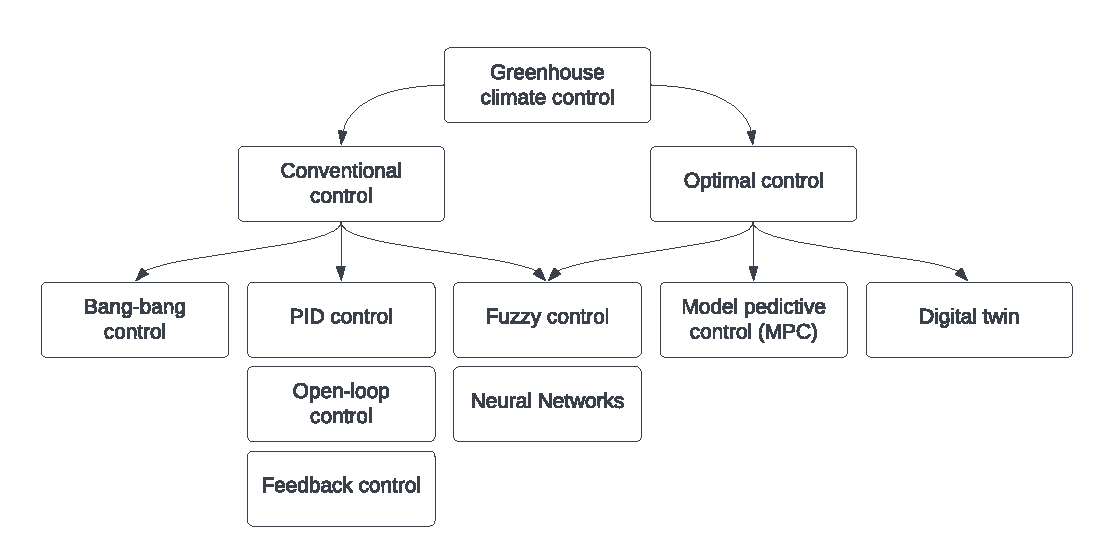
\includegraphics[width=.5\textwidth]{images/flowchart.pdf}
    \caption{A simplified diagram representing greenhouse control algorithms. Image adapted from \cite{10.1007/978-3-031-48649-4_13}.}
    \label{fig:flowchart}
\end{figure}

Adaptive control adjusts parameters based on real-time feedback \cite{Tian2022}, while nonlinear feedback control tackles system complexities with advanced algorithms \cite{Bood2023}. Fuzzy control addresses imprecise data and uncertainties \cite{smartcities7030055}, and robust control maintains stability despite disturbances \cite{Zhang2021}. Optimum control aims to fine-tune actions for best outcomes \cite{Debroy2024, SVENSEN2024108578}. However, these techniques often demand substantial computational power and intricate implementation, additionally, frequent adjustments raise energy consumption and actuator wear.

Consequently, PID controllers remained popular due to their simplicity and effectiveness. IoT and machine learning advancements are also enhancing greenhouse control, with Wang et al. \cite{Wang2024} combining these technologies with PID for real-time monitoring. Despite improvements, challenges accompany PID control due to the complexity of greenhouse systems requiring multiple controllers and extensive tuning. The process remains time-consuming and dependent on optimization, often without guaranteed optimal results. Therefore, MPC has gained traction in greenhouse climate control \cite{Hu2022}, however, opting for continuously adjusting parameter setpoints through online optimization on a sample-by-sample basis. This iterative optimization procedure can escalate computational load, thereby complicating system operation. 

% - Presentation of the studied methodology

% - Presentation of the problem
Effective greenhouse climate control involves various technologies, including cooling and heating systems such as fans and heaters. These and similar technologies are essential for maintaining optimal temperatures and improving energy efficiency.

% - Presentation of our contribution

% - Organization of the paper (optional; remove it if there is no space at the end)

\section{Methodology}

\begin{figure}
    \centering
    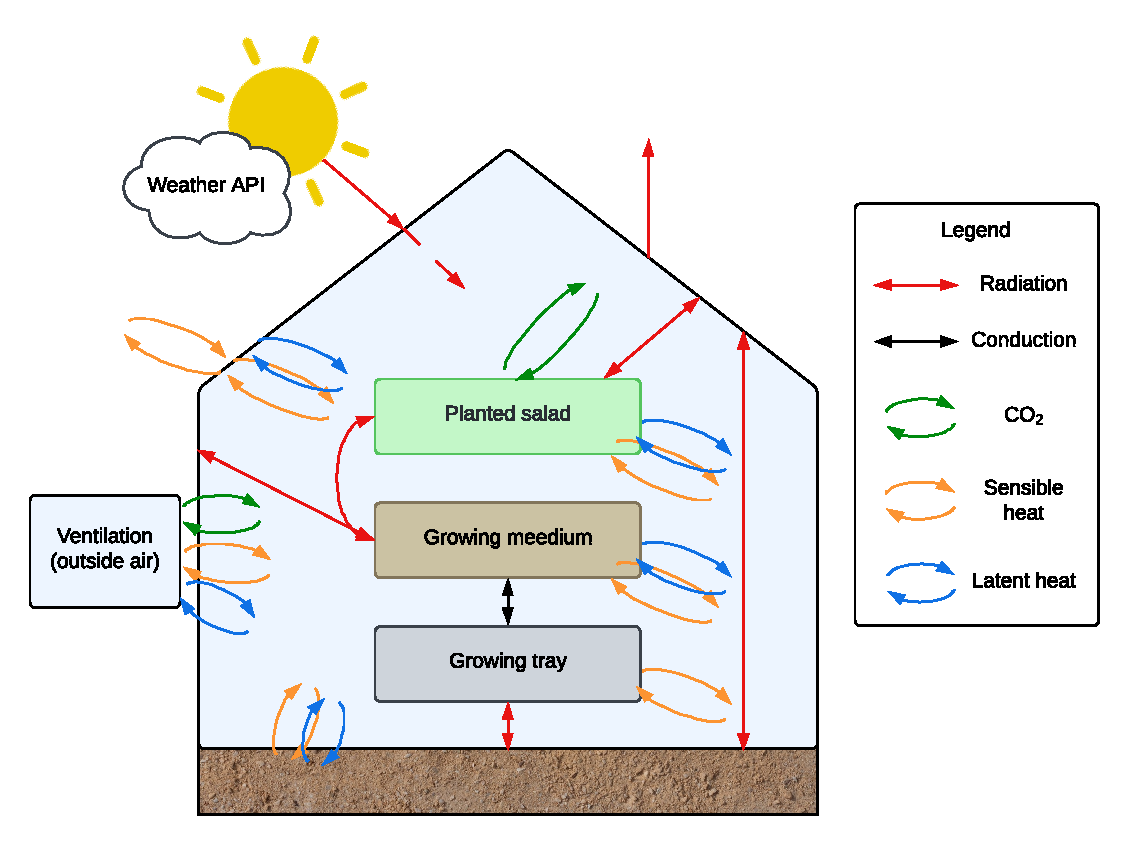
\includegraphics[width=.5\textwidth]{images/diagram.pdf}
    \caption{A simplified diagram of the heat, mass and CO2 exchanges modelled within the framework. Image adapted from \cite{rmward61_2019}.}
    \label{fig:diagram}
\end{figure}

\section{Results}

\section{Conclusion}

\bibliographystyle{IEEEtran}
\bibliography{main}

\end{document}
